\chapter{Fibre Bundles}\label{chapter:bundles}

    This chapter is formulated in sufficient generality so as to encompass both the topological and smooth setting (or any other one might find useful). To this end the generic terms ``space'', ``group'' and ``morphism'' are used. The reader should choose in which category he wants to work, e.g. topological space, topological group and continuous map in the case of $\mathbf{Top}$.

\section{Bundles}

    \newdef{Bundle}{\index{bundle}\label{diff:bundle}
        A triple $(E,B,\pi)$ where $E$ and $B$ are spaces and $\pi$ is a morphism. Sometimes one requires that the map $\pi$ is also surjective. However, under this additional restriction one cannot make the association $\mathbf{Bundle}(X)\cong\mathbf{C}/X$ of categories anymore.
    }

    An explicit example in the category $\mathbf{Diff}$ is the following:
    \begin{example}[Fibred manifold]\index{fibred!manifold}\index{fibre}
        A surjective submersion \ref{diff:submersion} \[\pi:E\rightarrow B,\] where $E$ is called the \textbf{total space}, $B$ the \textbf{base space} and $\pi$ the \textbf{projection}. For every point $p\in B$, the set $\pi^{-1}(p)$ is called the \textbf{fibre over $p$}.
    \end{example}

    The most important example of a bundle is a fibre bundle. Before being able to give the definition, an important tool needs to be introduced:
    \newdef{Cocycle}{\index{co-!cycle}\label{diff:G_cocycle}
        Let $B$ be a space and $G$ a group. A $G$-valued cocycle on $B$ with respect to an open cover $\{U_i\}_{i\in I}$ is a family of morphisms $g_{ij}:U_i\cap U_j\rightarrow G$ that satisfy the following condition (it is called the \textbf{\v{C}ech cocycle condition}):
        \begin{gather}
            \label{diff:G_cocycle_condition}
            g_{ij} = g_{ik}\circ g_{kj}.
        \end{gather}
        Two cocycles $(U_i,g_{ij})$ and $(V_i,h_{ij})$ are said to be equivalent if there exist morphisms $\lambda_{i,j}:U_i\cap V_j\rightarrow G$ such that
        \begin{gather}
            \lambda_{i,r}g_{ij}\lambda_{j,s}^{-1} = h_{rs}
        \end{gather}
        whenever this is well-defined. The resulting quotient set is denoted by $H^1(B;G)$.\footnote{The notation stems from the fact that this is the first \v{C}ech cohomology group with values in $G$ as explained in Section \ref{section:cech_de_rham}.}
    }
    \begin{property}\label{diff:G_cocycle_conditions}
        Let $\{g_{ij}\}_{i,j\in I}$ be a cocycle on $B$. It satisfies the following properties for all $x\in B$:
        \begin{itemize}
            \item $g_{ij}(x) = (g_{ji}(x))^{-1}$, and
            \item $g_{ii}(x) = e$.
        \end{itemize}
    \end{property}

    \newdef{Fibre bundle}{\index{fibre!bundle}\index{local!trivialization}\index{structure!group}
        \label{diff:fibre_bundle}
        A tuple $(E,B,\pi,F,G)$ where $E,B$ and $F$ are spaces and $G$ is a group (called the \textbf{structure group}), such that there exists a surjective morphism \[\pi:E\rightarrow B\] and an open cover $\{U_i\}_{i\in I}$ of $B$ together with a family of isomorphisms $\{\varphi_i:\pi^{-1}(U_i)\rightarrow U_i\times F\}_{i\in I}$ that make the following diagram commute for all $i\in I$:

        \begin{figure}[ht!]
            \centering
            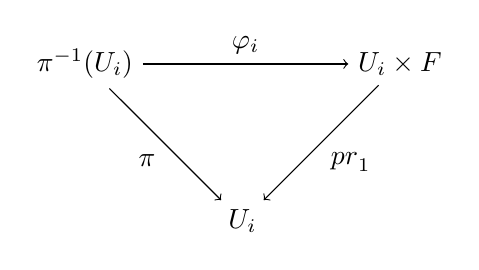
\begin{tikzpicture}
                \node (PI) at (-2, 0) {$\pi^{-1}(U_i)$};
                \node (UF) at (2, 0) {$U_i\times F$};
                \node (U) at (0, -2) {$U_i$};
                \draw[->] (PI) -- node[above]{$\varphi_i$} (UF);
                \draw[->] (PI) -- node[below left]{$\pi$} (U);
                \draw[->] (UF) -- node[below right]{$\text{pr}_1$} (U);
            \end{tikzpicture}
        \end{figure}
        As for general bundles one calls $E$ and $B$ the \textbf{total space} and \textbf{base space} respectively. The space $F$ is called the \textbf{(typical) fibre}. The pair $(U_i,\varphi_i)$ is sometimes called a \textbf{bundle chart} and the set $\{(U_i,\varphi_i)\}_{i\in I}$ is often called a \textbf{local trivialization}\footnote{This name follows from the fact that the bundle is locally isomorphic to a (trivial) product space: $E\cong U\times F$.}. The cover $\{U_i\}_{i\in I}$ itself is called a \textbf{trivializing cover} of the bundle.

        The \textbf{transition maps} $\varphi_j\circ\varphi_i^{-1}:(U_i\cap U_j)\times F\rightarrow (U_i\cap U_j)\times F$ can be identified with the cocycle $g_{ji}:U_i\cap U_j\rightarrow G$, associated to the (left) action (which is required to be faithful\footnote{See definition \ref{group:faithful_action}.}) of $G$ on every fibre, by the following relation:
        \begin{gather}
            \varphi_j\circ\varphi_i^{-1}(b, x) = (b, g_{ji}(b)\cdot x).
        \end{gather}
    }
    \begin{remark}
        One should pay attention to the fact that the bundle charts are not coordinate charts in the sense of manifolds \ref{diff:chart} because the image of $\varphi_i$ is not an open subset of $\mathbb{R}^n$. However, they serve the same purpose as they are used to locally describe the total space $P$.
    \end{remark}
    \begin{notation}
        A fibre bundle $(E,B,\pi,F,G)$ is often denoted by $F\hookrightarrow E\xrightarrow{\ \pi\ }{B}$ or even $\pi:E\rightarrow B$ if the fibre is not important. A drawback of such notations is that the structure group of the bundle is not shown.
    \end{notation}

    \newdef{Numerable fibre bundle}{\index{numerable}\label{diff:numerable_bundle}
        A fibre bundle that admits a local trivialization over a numerable open cover.
    }

    \newdef{Compatible\footnotemark\ bundle charts}{\index{compatible!bundle charts}
        \footnotetext{Also called an \textbf{admissible chart}.}
        A bundle chart $(V,\psi)$ is said to be compatible with a trivializing cover $\{(U_i,\varphi_i)\}_{i\in I}$ if whenever $V\cap U_i\neq\emptyset$, there exists a map $h_i:V\cap U_i\rightarrow G$ such that
        \begin{gather}
            \psi\circ\varphi_i^{-1}(b,x) = (b,h_i(b)x)
        \end{gather}
        for all $b\in V\cap U_i$ and $x\in F$. Two trivializing covers are said to be equivalent if all bundle charts are cross-compatible. As in the case of manifolds, this gives rise to the notion of a \textbf{$G$-atlas}. A \textbf{$G$-bundle} is then defined as a fibre bundle eqipped with an equivalence class of $G$-atlases.
    }

\section{Bundle maps}

    \newdef{Bundle map}{\index{bundle!map}
        A bundle map between two fibre bundles $\pi_1:E_1\rightarrow B_1$ and $\pi_2:E_2\rightarrow B_2$ is a pair $(f_E,f_B)$ of morphisms that make diagram \ref{fig:bundle_map} commute. The map $f_E$ is said to \textbf{cover} $f_B$. If such a couple exists, the base map $f_B$ is uniquely determined by $f_E$ and therefore a bundle map is often just denoted by $f_E:E_1\rightarrow E_2$.

        \begin{figure}[ht!]
        \centering
        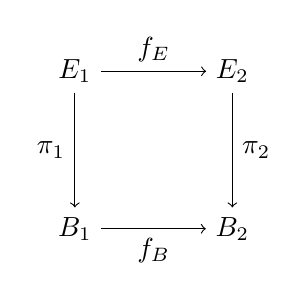
\begin{tikzpicture}
            \node (E1) at (0, 0) {$E_1$};
            \node (E2) at (2, 0) {$E_2$};
            \node (B1) at (0, -2) {$B_1$};
            \node (B2) at (2, -2) {$B_2$};
            \draw[->] (E1) -- node[above]{$f_E$} (E2);
            \draw[->] (E1) -- node[left]{$\pi_1$} (B1);
            \draw[->] (E2) -- node[right]{$\pi_2$} (B2);
            \draw[->] (B1) -- node[below]{$f_B$} (B2);
        \end{tikzpicture}
        \caption{Bundle map between fibre bundles.}
        \label{fig:bundle_map}
        \end{figure}
    }
    \newdef{Isomorphism}{
        Two fibre bundles $F$ and $G$ are said to be isomorphic if there exist bundle maps $f:F\rightarrow G$ and $g:G\rightarrow F$ such that $f\circ g = \mathbbm{1}_G$ and $g\circ f = \mathbbm{1}_F$.
    }

    \newdef{Equivalent fibre bundles}{\index{gauge!transformation}
        Two fibre bundles $\pi_1:E_1\rightarrow B$ and $\pi_2:E_2\rightarrow B$, with the same typical fibre and structure group, are said to be equivalent if there exist trivializations\footnote{Remark that the collection $\{U_i\}_{i\in I}$ is the same for both trivializations.} $\{(U_i,\varphi_i)\}_{i\in I}$ and $\{(U_i,\varphi'_i)\}_{i\in I}$ such that the associated cocycles are equivalent. An explicit form of the functions $\lambda$ is given by
        \begin{gather}
            \lambda_{i,i} := \varphi_i'\circ\varphi_i^{-1}.
        \end{gather}
    }
    \begin{property}
        Two fibre bundles over the same base space are equivalent if and only if they are isomorphic.
    \end{property}

    \newdef{Trivial bundle}{\index{trivial}\label{diff:trivial_bundle}
        A fibre bundle $(E,B,\pi,F)$ is said to be trivial if there exists an equivalence $E\cong B\times F$.
    }

\section{Constructions}

    \begin{construct}[Fibre bundle construction theorem]\label{diff:fibre_bundle_construction_theorem}
        Let $M$ and $F$ be spaces and let $G$ be a group equipped with a left action on $F$. Suppose that a cover $\{U_i\}_{i\in I}$ of $M$ and a collection of morphisms $\{g_{ji}:U_i\cap U_j\rightarrow G\}$ that satisfy the cocycle condition \ref{diff:G_cocycle} are given. A fibre bundle over $M$ can then be constructed as follows:
        \begin{enumerate}
            \item First construct for every set $U_i$ an associated set $U_i\times F$.
            \item Then construct the disjoint union $T:=\bigsqcup_{i\in I}U_i\times F$ and equip it with the disjoint union topology (see definition \ref{topology:disjoint_union}).
            \item From this disjoint union construct a quotient space and equip it with the quotient space topology (see definition \ref{topology:quotient_space}) induced by the following equivalence relation for every $i,j\in I$:
                \begin{gather}
                    (p, f)\sim(p,g_{ji}(x)\cdot f)
                \end{gather}
                for all $x\in U_i\cap U_j$ and $f\in F$.
            \item The fibre bundle is equal to the quotient space $T/\sim$ equipped with the projection $\pi$ that maps the equivalence class $(x,f)\in T$ to $x\in M$.
            \item Local trivializations are given by the maps $\varphi_i:\pi^{-1}(U_i)\rightarrow U_i\times F$ that satisfy
                \begin{gather}
                    \varphi_i^{-1}:(x,f)\mapsto [(x,f)],
                \end{gather}
                where $[A]$ denotes the equivalence class of $A$ in $T/\sim$.
        \end{enumerate}
    \end{construct}
    \begin{property}[Homotopy invariance]
        Homotopic transition functions give rise to equivalent (and hence isomorphic) bundles. (This follows from the homotopy invariance of \v{C}ech cohomology.)
    \end{property}

    \begin{remark}[Clutching]\index{clutching}
        The above construction is often called the clutching construction, especially when constructing vector bundles over a sphere $S^n$. There the covering consists of two hemispheres that intersect on the equator $S^{n-1}$ and the function $g_{21}$ is in that case also called the \textbf{clutching function}.
    \end{remark}
    \begin{property}[Vector bundles over a sphere]\index{vector!bundle}\label{diff:vector_bundles_over_sphere}
        The clutching theorem and the homotopy invariance imply that vector bundles over the sphere are determined by homotopy classes of functions $S^{n-1}\rightarrow\text{GL}_p(k)$, i.e. they are classified by the homotopy group $\pi_{n-1}(\text{GL}_p(k))$.
    \end{property}

    \newdef{Subbundle}{\index{sub!bundle}
        A subbundle of a fibre bundle $\pi:E\rightarrow B$ is a triple $(E',B',\pi')$ such that $E'\subset E$, $B'\subset B$ and $\pi' = \pi|_{E'}$.
    }
    \newdef{Pullback bundle}{\index{pullback!bundle}\label{diff:pullback_bundle}
        Let $\pi:E\rightarrow B$ be a fibre bundle and let $f:B'\rightarrow B$ be a morphism of spaces. The total space of the pullback bundle $f^*E$ is defined as follows:
        \begin{gather}
            f^*E := \big\{(b',e)\in B'\times E:f(b') = \pi(e)\big\}.
        \end{gather}
        The topology on $f^*E$ is induced by the subspace topology of the product $B'\times E$. The projection onto the second factor gives a map of total spaces $f^*E\rightarrow E$.
    }

    \newdef{Fibre product}{\index{fibre!product}
        Let $(F_1,B,\pi_1)$ and $(F_2,B,\pi_2)$  be two fibre bundles over the same base space $B$. Their fibre product is defined as follows:
        \begin{gather}
            \label{diff:fibre_product}
            F_1\diamond F_2 := \big\{(f, g)\in F_1\times F_2: \pi_1(f) = \pi_2(g)\big\}.
        \end{gather}
    }

\section{Sections}

    \newdef{Section}{\index{section}
        A (\textbf{global}) section of a fibre bundle $\pi:E\rightarrow B$ is a morphism $s:B\rightarrow E$ such that $\pi\circ s = \mathbbm{1}_B$. For any open subset $U\subset B$ a \textbf{local} section is defined as a morphism $s_U:U\rightarrow E$ such that $\pi\circ s_U(b) = b$ for all $b\in U$.
    }
    \begin{notation}
        \nomenclature[O_Gamma]{$\Gamma(E)$}{set of global sections of a fibre bundle $E$}
        The set of all global sections of a bundle $E$ is denoted by $\Gamma(E)$. The set of local sections over $U$ is sometimes denoted by $\Gamma(U, E)$. With this latter notation one also has $\Gamma(E)\equiv\Gamma(B, E)$.
    \end{notation}

    \begin{property}[Pullback of sections]
        The sections of a fibre bundle $E$ pullback to the pullback bundle $f^*E$ by setting $f^*s := s\circ f$.
    \end{property}